\documentclass[a4paper, 11pt]{article}
\usepackage{fullpage}

\usepackage[utf8]{inputenc}
\usepackage[swedish]{babel}

\usepackage{amsmath}
\usepackage{amsfonts}
\usepackage{amssymb}
\usepackage{graphicx}
\usepackage{float}
\usepackage{listings}
\usepackage{multirow}
\usepackage{fontenc}

\usepackage[hidelinks]{hyperref}

\usepackage{titlesec}
\setcounter{secnumdepth}{4}

\usepackage[backend=biber,style=numeric,sorting=none]{biblatex}
\addbibresource{cites.bib}

\usepackage{caption}
\captionsetup[figure]{name=Figur}

\begin{document}

\begin{titlepage}
\newcommand{\HRule}{\rule{\linewidth}{0.5mm}}
\begin{center}

\textsc{\Large }\\[2.5cm]
\textsc{\LARGE Uppsala Universitet}\\[1.5cm] 

\HRule \\[0.3cm]
{ \huge \textup {Historiekunskapsspel med semiautomatisk frågehämtning och ett balanseringssystem för frågor}}\\[0.3cm]
\HRule \\[1.5cm]


\Large \textsc{Författare:}\\[0.5cm]
\end{center}
\begin{minipage}{0.4\textwidth}
\begin{flushleft} \large
\large \textup{Alfred Yrelin}\\
\large \textup{Alfred.Yrelin.2125@student.uu.se}\\
\large \textup{\textup{Inst. för informationsteknolog}}\\
\large \textup{\textup{Uppsala Universitet}}
\end{flushleft}
\end{minipage}
~ \hfill
\begin{minipage}{0.4\textwidth}
\begin{flushright} \large
\large \textup{Josef Svensson}\\
\large \textup{Josef.Svensson.8440@student.uu.se}\\
\large \textup{\textup{Inst. för informationsteknologi}}\\
\large \textup{\textup{Uppsala Universitet}}
\end{flushright}
\end{minipage}

\center

\begin{minipage}{0.4\textwidth}
\large \textup{Philip Åkerfeldt}\\
\large \textup{Philip.Akerfeldt.4987@student.uu.se}\\
\large \textup{\textup{Inst. för informationsteknolog}}\\
\large \textup{\textup{Uppsala Universitet}}
\end{minipage}\\ [1.5cm]
~
{\Large \today}\\[2cm]
\vfill

\end{titlepage}

%\maketitle
\newpage
\section{Förord}
\textit{Tack till}
\newpage
\tableofcontents
\pagebreak

\section{Inledning}
Vem vill inte kunna avgöra diskussioner med sina vänner med argumentet "Jag är i alla fall bäst på ..."? 
Att tävla är både en rolig och en social aktivitet. Oavsett om målet är att vinna eller bara ha kul så bidrar spel ofta med någon form av tävlingskänsla. Att kunna få denna tävlingskänsla och samtidigt en källa för nöje så förmånligt i sin telefon är något som vi tror är något att eftersträva i mobila spel. Spel som exempelvis Quizkampen \cite{quiz} och Wordfeud \cite{wordfeud} besitter båda denna egenskap och det är därför vi tror att dessa spel har blivit så populära på marknaden \cite{appsalesrating}. Vi eftersträvar att skapa ett spel som kan framkalla samma tävlingskänsla och nöje som Quizkampen och Wordfeud. Ett spel som går ut på att ordna historiska händelser relativt till andra händelser. 

Applikationsutveckling för mobila enheter är ett spännande område som växer \cite{IDC}, under sista kvartalet av 2014 hade Android 81,5\% av marknaden och av de enheter som såldes hade 76,6\% Android som operativsystem. Enligt Digi-Capital-Found \cite{revenue} var även Android operativsystemet som gav högst intäkter för utvecklare som placerat sina applikation i någon form av applikationsmarknad, även om intäkter per nerladdning i iOS fortfarande var större. \\

VÅRT SPEL utvecklas till Android med en backend som drar nytta av Google App Engines skalbarhet för att ge applikationen möjlighet att växa i takt med användarantalet. För att inte behöva söka och manuellt lägga in ett stort antal frågor utvecklas en semi-automatisk frågehämtare. Detta bidrar till att VÅRT SPEL inte blir repetitivt och tråkigt för användarna. Frågehämtaren möjliggör att frågorna kan läggas in utan att utvecklarna behöver lägga mycket tid på det. En annan sak som gjordes för att spelet skulle vara roligare för alla var att skapa ett balanseringssystem som gör att händelserna som ges till spelarna är anpassade efter hens kunskapsnivå.


\section{Förutsättningar}

\subsection{Bakgrund}

\subsubsection{Kunskapsspel för mobiltelefoner}
Wordfeud och Quizkampen är två populära turbaserade multiplayerspel där Quizkampen har 45 miljoner användare globalt \cite{quiz} och Wordfeud har 20 miljoner användare \cite{wordfeud}. Dessa spel gör det möjligt att utmana vänner eller slumpmässiga personer på en match som spelas i omgångar. När en spelare spelar sin omgång får dess motståndare vänta på sin tur, vilket gör att en match kan pågå i flera dagar.

\paragraph{Quizkampen \newline} 
Quizkampen \cite{aboutquiz} är ett frågesports-spel där spelarna svarar på frågor under 6 rundor med tre frågor i varje runda. Spelarna svarar på samma frågor varje runda.  Inför varje runda slumpas tre kategorier fram där endast en kategori väljs för den aktuella rundan. Valet av kategorier är något som spelarna turas om att göra varannan runda. Matchen avslutas när sista rundan är spelad och det är även då en vinnare koras beroende på vem som har flest poäng. 

\paragraph{Wordfeud \newline}
Wordfeud \cite{aboutwordfeud} är ett spel där en match utspelas mellan två personer. Varje spelare får en liten mängd bokstäver som är gömd för motspelaren. Spelet går sedan ut på att fläta samman ord på det givna spelbrädet med hjälp av bokstäverna. Målet är att få så många poäng som möjligt och detta kan man uppnå tack vare att varje bokstav är värd en viss poäng. På så sätt kan man genom att använda svårare bokstäver och skapa längre ord få mer poäng. 

\subsubsection{Sällskapsspel med fokus på kunskap}
Sällskapsspel har länge varit och är än idag ett populärt sätt att umgås på \cite{bradspelspop}. Sällskapsspelet \textit{När då då?} \cite{nardada} är ett spel har bygger på ett relativt enkelt koncept. Spelarna turas om att placera ut händelser på en tidslinje i förhållande till varandra och får poäng om dessa är korrekt utplacerade. Den spelaren som har flest poäng vid en slutet av matchen vinner. \\
Spelkonceptet är som sagt ett enkelt sådant men det är också kraftfullt i den meningen att det främjar vissa begär hos spelarna. Ett av begären är att man vill överkomma problem som ställs av antingen spelet själv eller motspelarna. Detta är en av faktorerna som gör den typen av spel så populära \cite{psykologi}.

\subsection{Syfte}
Det är projektets syfte är att utveckla och distribuera en spelapplikation för mobila enheter som använder plattformen Android. I det här projektet ska en applikation utvecklas som ska ge flera användare möjlighet att interagera och spela med varandra.

Spelet som utvecklats går ut på att två användare får tävla om vem som har bäst koll på när olika historiska händelser ägde rum. Varje spelare får ett antal händelser som hen sedan ska sortera i kronologisk ordning. Spelaren som sorterar flest händelser rätt vinner. Förutom rent nöje så kan spelet användas i utbildningssyfte. Detta i den meningen att det ger användaren en ypperlig möjlighet att förbättra sina kunskaper om historien.

\subsection{Mål}
Det finns fyra stora delar i det här projektet som kan ses som projektets primära fokuspunkter. Målet vi har för avsikt att uppnå är en mobilapplikation i form av ett spel. Spelet skall köras på en server som ska sköta all kommunikation mellan klienten och sig själv. En av de primära fokuspunkterna för spelet är att implementera en semi-automatisk informationshämtare som har som ska fylla på spelets databas med nya frågor. Att informationshämtningen är semi-automatiskt betyder att ett steg i informationshämtningen kräver mänsklig interaktion. Interaktionen krävs för att godkänna frågorna till databasen och detta är en uppgift som administratörerna (se avsnitt \ref{admins}) utför. 


\subsubsection{Mobilapplikation}
Vi strävar mot att utveckla en mobilapplikation till Android. Applikationen är det enda som användaren i slutändan ser och därför finner vi att kvaliteten av gränssnittet är extra viktigt i utvecklingen. 

Applikationen till Android skrivs i Java och gränssnittet skrivs med hjälp av XML \cite{xml}. 

\subsubsection{Server}
För att flera spelare ska kunna interagera med varandra så behövs det en server. En server möjliggör även att frågorna i spelet kan uppdateras kontinuerligt under applikationens exekvering.

Servermjukvaran skrivs i programspråket Go \cite{golang} och körs på Googles molntjänst App Engine.

\subsubsection{Google App Engine} 
Google App Engine är en \textit{Platform as a service}, vilket är en servicemodell för molntjänster. Det bygger på att användaren skapar en programvara med hjälp av färdigbyggda bibliotek och verktyg som leverantören tillhandahåller. Programmet man bygger i App Engine körs på Googles infrastruktur och är uppbyggt så att man kan utöka antalet användare obegränsat. Flera stora företag har använt sig av App Engine när de lanserat produkter bland annat Coca Cola, Rovio och Best Buy \cite{googleappenginecustomers}. 

\subsubsection{Automatisk informationshämtning}
För att göra spelet så intressant som möjligt behövas en stor bredd på frågorna som finns lagrade i spelets tillhörande databas. Ett sätt att skapa många frågor snabbt är att utveckla mjukvara som kan hämta information och från denna informationen skapa nya frågor automatiskt. 

Målet med den automatiska informationshämtningen är att skapa ett delsystem som läser in delar av en hemsida, som följer en viss struktur, för att hitta nödvändig information. Systemet koppla sedan samman årtalen och händelserna från hemsidan automatiskt. Det här systemet behöver också ett gränssnitt för att ge administratörerna ett snabbt sätt att korrekturläsa frågorna innan de godkänns och skickas vidare till spelet. För mer detaljerad information om mjukvarans design se avsnitt \ref{crawler}.

\subsection{Motivation}
Det finns många mobilspel som handlar om att två personer möts och mäter sina färdigheter inom ett visst område. Exempel på sådana applikationer är Quizkampen och Wordfeud som båda toppar säljlistorna för Androidspel \cite{appsalesrating}. Dessa spel följer en ganska enkel struktur och den bygger på att två personer kan möta varandra, svara på frågor eller lägga ord korrekt. På detta sätt får spelarna poäng som sen avgör vinnaren mellan de tävlande. Enligt säljstatistiken \cite{appsalesrating} är detta koncept något som är attraktivt för många användare. Spelet, vars utveckling beskrivs i rapporten, kombinerar koncepten från Quizkampen och Wordfeud i den mening att spelare ska svara på frågor samt att lägga in saker på sin rätta plats. 

En liknande version av det här spelet har också visat sig vara populär i form av sällskapsspel (\textit{När-då-då?}) \cite{nardada}. Detta är en av anledningarna till att hoppet är stort att även den här applikationen ska bli populär på marknaden. Det finns för tillfället ingen variant av det här spelkonceptet till Android vilket ses som en bra chans att ta enligt utvecklingsteamet.

\subsection{Relaterat arbete}
Det finns ett spel för iOS, \textit{Historiekampen} \cite{historiekampen} som också handlar om att lägga in händelser korrekt på en tidslinje. En nackdel som den befintliga iOS-versionen har är att användaren endast ser årtal på sin tidslinje, och inte vilka händelser som ligger där.

\subsubsection{Historiekampen}
Historiekampen är ett spel som konceptuellt sett liknar sällskapsspelet \textit{När då då?} väldigt mycket. En spelares tur går till så att denne först får en händelse som ska placeras på spelarens tidslinje. När första frågan presenteras finns det en årtalsreferens utlagd på tidslinjen som den första händelsen ska placeras före eller efter. När nästa fråga presenteras finns det två referenser (den första plus årtalet för frågan som precis placerades) och så vidare.\\ 
Historiekampen har valt att använda konceptet med kombinations-poäng vilket betyder att spelaren kan få flera poäng under en runda om hen placerar ut flera händelser korrekt efter varandra. Spelaren måste placera minst \underline{en} händelse och kan få maximalt tio händelser att placera ut. Om spelaren placerar första händelsen fel är rundan avslutad men om spelaren placerar händelsen rätt ställs hen inför ett val med två alternativ: antingen avsluta sin runda och på så sätt låsa sina poäng, eller fortsätta att få händelser att placera ut i förhållande till de tidigare händelserna. Detta val gör spelaren efter varje rätt placerad händelse. Spelaren kan med andra ord välja själv om den vågar fortsätta eller om den vill vara försiktig och behålla sina välförtjänta poäng. En duktig spelare kan välja det senare alternativet och bygga upp sin kombo fram tills dess att den femte frågan är ställd. När den femte frågan är ställd får hen en fråga om \underline{när} den femte händelsen ägde rum. Om spelarens svar är nära det rätta årtalet får hen fortsätta rundan med sin uppbyggda kombo av poäng. Om årtalet är fel förlorar spelaren sina tidigare poäng men kan fortsätta få händelser att placera ut till de tidigare händelserna. Vid en perfekt runda kan en spelare få totalt tio poäng.

\subsubsection{Balanseringsteori}
En viktig aspekt i det här projektet är att rangordna spelare i förhållande till varandra för att med hjälp av det skapa mer rättvisa matcher. Den här problematiken finns det redan många som har funderat på och de flesta större spel använder sig också av något system för detta. Två etablerade system är Elo och Glicko, varav Elo är det som har implementerats i det här projektet.

Elo är ett system som förutser hur stor del av en mängd spelade matcher som bör vinnas av vardera spelare, baserat på en den svårighetsnivå respektive spelare har. Det här systemet justerar, efter en match, poängen enligt beskrivningen ovan. Eftersom en lägre rankad spelare får fler poäng vid vinst mot en högre rättar systemet på sikt sig självt, vilket innebär att spelarna faktiskt får den nivå de förtjänar.

Elo-systemet fungerar enligt följande. Varje spelare får en initial Elo-poäng på 1000. Denna justeras sedan beroende på utfallet av en match i förhållande till det förväntade utfallet. Det förväntade utfallet beräknas:

$$E_A = \frac{1}{1+10^{(R_B-R_A)/400}}$$

Där $E_A$ är den förväntade andelen matcher som spelare A borde vinna. Är värdet till exempel 0.84 så innebär det att 84\% av matcherna borde vinnas av spelare A enligt nuvarande Elo-poäng. $R_B$ är spelare B:s nuvarande Elo-poäng och $R_A$ är spelare A:s nuvarande poäng.

När det förväntade utfallet har beräknats så justeras sedan spelarnas Elo-poäng enligt formeln:

$$R'_A = R_A + K(S_A-E_A)$$

Där $R'_A$ är spelare A:s nya Elo-poäng, $R_A$ är spelare A:s Elo-poäng innan matchen, $S_A$ är det faktiska utfallet av matchen och $E_A$ är det förväntade utfallet. K-värdet är en skalningsfaktor som justerar hur mycket poängen justeras vid varje vinst/förlust.

Ett räkneexempel med spelare A, 1300 poäng, och spelare B 1000 poäng, där A vinner:

$$0.849 = \frac{1}{1+10^{(1000-1300)/400}}$$
$$ R'_A = 1300 + 16(1-0.849) = 1302.416 $$
$$ R'_B = 1000 + 16(0-0.849) = 997.584 $$

I det implementerade balanseringssystemet används Elo-modellen för att beräkna spelarnas erfarenhetspoäng. Elo är ett system som utvecklades av Arpad Elo och började användas redan på 60-talet\cite{elo}. Systemet var först och främst utvecklat för att ranka schackspelare, men har sedan dess uppkomst även applicerats på många andra spel. Eftersom Elo-systemet är förhållandevis gammalt och möjligheten till datoriserade beräkningar blivit större sedan 60-talet, finns det mer avancerade system att använda sig av idag. Ett annat system som utvecklades i syfte att vara en förbättring av Elo-systemet är ett system kallat Glicko\cite{chessratings}. Skillnaden mellan Elo och Glicko är att Glicko också har ett värde för hur väl uppdaterad spelarens erfarenhetspoäng är. Det här innebär att spelaren har ett erfarenhetspoäng, säg 2000, samt ett trovärdighetspoäng, till exempel 100. Ju högre trovärdighetspoäng spelaren har, desto mindre exakt är erfarenhetspoängen. Erfarenhetspoängen har enligt systemet en +/- diff på dubbla trovärdighetspoängen. I nyss nämnda exempel innebär detta att spelaren har en erfarenhetspoäng på 1800-2200. Trovärdighetspoängen justeras bland annat baserat på hur länge sedan det var spelaren spelade förra gången, samt hur många matcher spelaren spelat totalt. Ju fler matcher totalt och ju närmare i tid förra matchen var, desto lägre trovärdighetspoäng har spelaren.

Både Elo och Glicko används idag och det verkar vara svårt att avgöra om Glicko verkligen är bättre än Elo\cite{stackchess}. Ett faktum som finns är i alla fall att Glicko kräver mer information för att kunna fungera. En faktor som Glicko behöver men inte Elo är en tidsvariabel som har reda på hur länge sedan det var spelaren spelade sin förra match\cite{glickoex}. Det här gör att mer data behöver lagras i databasen, vilket är negativt ur kapacitetsperspektiv.

\subsection{Faktorer som gör VÅRT SPEL unikt i förhållande till konkurrenterna}
VÅRT SPEL liknar Historiekampen och \textit{När då då?} rent konceptuellt. Uppgiften som spelarna ska utföra i vår applikation liknar varandra mycket. I både Historiekampen och VÅRT SPEL är det spelarens uppgift att placera ut händelser rätt på en tidslinje. Spelmekaniken är dock annorlunda i vår applikation då varje match och varje runda behandlas annorlunda. I \textbf{VÅRT SPEL} får varje spelare ett paket med sex frågor varje runda. En av dessa sex frågor kommer agera som referenshändelse på tidlinjen. Frågorna presenteras för spelaren en i taget och det är sedan spelarens uppgift att placera dessa i rätt ordning. En spelare får ett poäng per korrekt utplacerad händelse och kan på så sätt på maximalt fem poäng från de korrekt placerade händelserna. Om en spelare skulle lyckas få en perfekt runda, där alla händelser placerades rätt, får hen ett extra poäng vilket skulle resultera i en total summa av sex poäng. Likt Historiekampen avslutas en runda när en spelare har placerat en händelse fel. Det som skiljer vår applikation i denna aspekt är vid fallet då en spelare har tjänat ihop poäng från tidigare händelser. I Historiekampen förlorar spelaren alla sina tidigare poäng om hen svarar fel medan i vår applikation får spelaren behålla sina poäng. Oavsett om spelaren lyckas placera ut alla händelser rätt eller inte så går turen, efter fem frågor, över till motståndaren. När fem rundor har spelats vinner den spelare som har svarat rätt på flest frågor totalt.  

En viktig detalj som skiljer VÅRT SPEL från Historiekampen är faktumet att spelaren ser beskrivningen av händelserna som hen placerat tidigare istället för bara årtalen. Vid avslutad runda visas även de korrekta årtalen för händelserna så att spelaren vet vilken ordning som hade varit den korrekta. \textbf{VÅRT SPEL} handlar med andra ord mer om att relatera händelser till varandra (dog Palme efter andra världskriget?) istället för att veta vilket årtal det skedde.

Med den semi-automatiska frågehämtaren, som kan anpassas för olika informationskällor, är det enkelt för utvecklarna att hämta nya frågor. Databasen med frågor kan på så sätt expandera snabbt vid behov. Detta är något som skiljer oss från Historiekampen där alla frågor matas in manuellt. \\
Vår applikationen balanserar även frågorna kontinuerligt efter varje match vilket bidrar till att alla spelare ska presenteras med frågor som passar deras aktuella kunskapsnivå. Balanseringen i spelet kan även byggas ut och göras mer avancerad om användarna skulle ge kritik på hur frågorna rankas. Det finns egentligen inga gränser för hur avancerad balansering kan göras vilket är en stor fördel som skiljer oss från konkurrenterna. För att läsa mer om balanseringen se avsnitt \ref{balanseringssystemet}.

\subsection{Frågeställningar}

\subsubsection{Tekniska problem}
Det finns vissa delar i det här systemet som blir mer avancerade att lösa än andra delar. Här listas några av dessa.
\begin{itemize}
\item Eftersom applikationen på något sätt ska hämta information och konstruera frågor på ett semi-automatiskt sätt måste ett sådant system utvecklas. En svårighet i detta är att se till att systemet blir tillräckligt smart för att lyckas läsa en informationskälla och ta ut den eftertraktade informationen på rätt sätt.
\item Det behövs en relativt stor databas för att lagra både användare och frågor för spelet. Det här är någonting som utvecklarna inte har arbetat med på en stor skala förut. Hur ska man lagra all information på ett sätt som är båda effektivt att lagra samt snabbt och enkelt för servern att hämta?
\item Det krävs nätverkskommunikation med säkerhet och användaridentifiering. App Engine som används vid stora delar av utveckling har användbara funktioner som uppfyller vissa delar men inte alla. Hur ska utvecklarna lyckas tillgodose användarna med en säker applikation?
\item Spelet ska anpassa svårighetsgraden automatiskt vilket betyder att någon form av balansering krävs. Tanken är att frågorna ska ha en svårighetsgrad som justeras automatiskt beroende på hur ofta de läggs rätt. Här måste det också tas hänsyn till hur resten av brädet ser ut vid tillfället. Hur skall detta utvecklas på ett tillräckligt effektivt och rättvist sätt för applikationen och användarna.
\item Det finns ett behov av att utveckla ett system för att rangordna spelare i någon slags topplista. Hur skall detta ske och hur kommer rangordningen bestämmas utifrån spelets mekanik? 
\end{itemize}

\section{Genomförande}

\subsection{Metoder}
Ett antal olika verktyg används för att möjliggöra detta projekt. För utvecklingen och simulering av Android-applikationen kommer Android Studio \cite{androidstudio} användas. Detta är ett kraftfullt verktyg som på ett smidigt sätt kan simulera applikationen i olika valbara miljöer i form av layouts för olika mobiltelefoner.\\
Google App Engine används lokalt för att simulera serverapplikationen. I skarpt läge kommer App Engine även användas, men då i Googles moln. App engine är ett värdefullt verktyg i vår utveckling med den enkla förklaringen att de tjänster som erbjuds när man utvecklar och körs sina applikationer via denna motor är otroligt värdefulla. Det är bland annat lätt att underhålla applikationen och skala när trafiken och datan kräver det  \cite{googleappengine}.\\
Den primära källan för information till frågorna har under utvecklingsfasen varit Wikipedia men denna ska bytas ut mot andra informationskällor vid ett senare skede. Detta skulle exempelvis vara innan produkten färdigställs.\\ 
Valet att inte använda Wikipedia som informationskälla i den slutgiltiga versionen av applikationen beror på dess tvivelaktiga roll som en pålitlig källa. Wikipedia trovärdighet har länge diskuterats och det finns många rapporter som har undersökt dess trovärdighet. Faktumet att processen för att skapa och redigera artiklar på Wikipedia idag anses vara något osäker. Detta beror mycket på att hemsidan följer strukturen \textit{editable-by-all} vilket betyder att vem som helst kan ändra artiklar och på så sätt vinkla artikeln innehåll. Detta betyder såklart inte att alla artiklar har råkat ut för detta öde men det bidrar till en viss osäkerhet vid användande av denna hemsida som källa vid vetenskapliga rapporter \cite{wikipediacred}.\\

\subsection{Systemstruktur}

\begin{figure}[H]
	\begin{centering}
	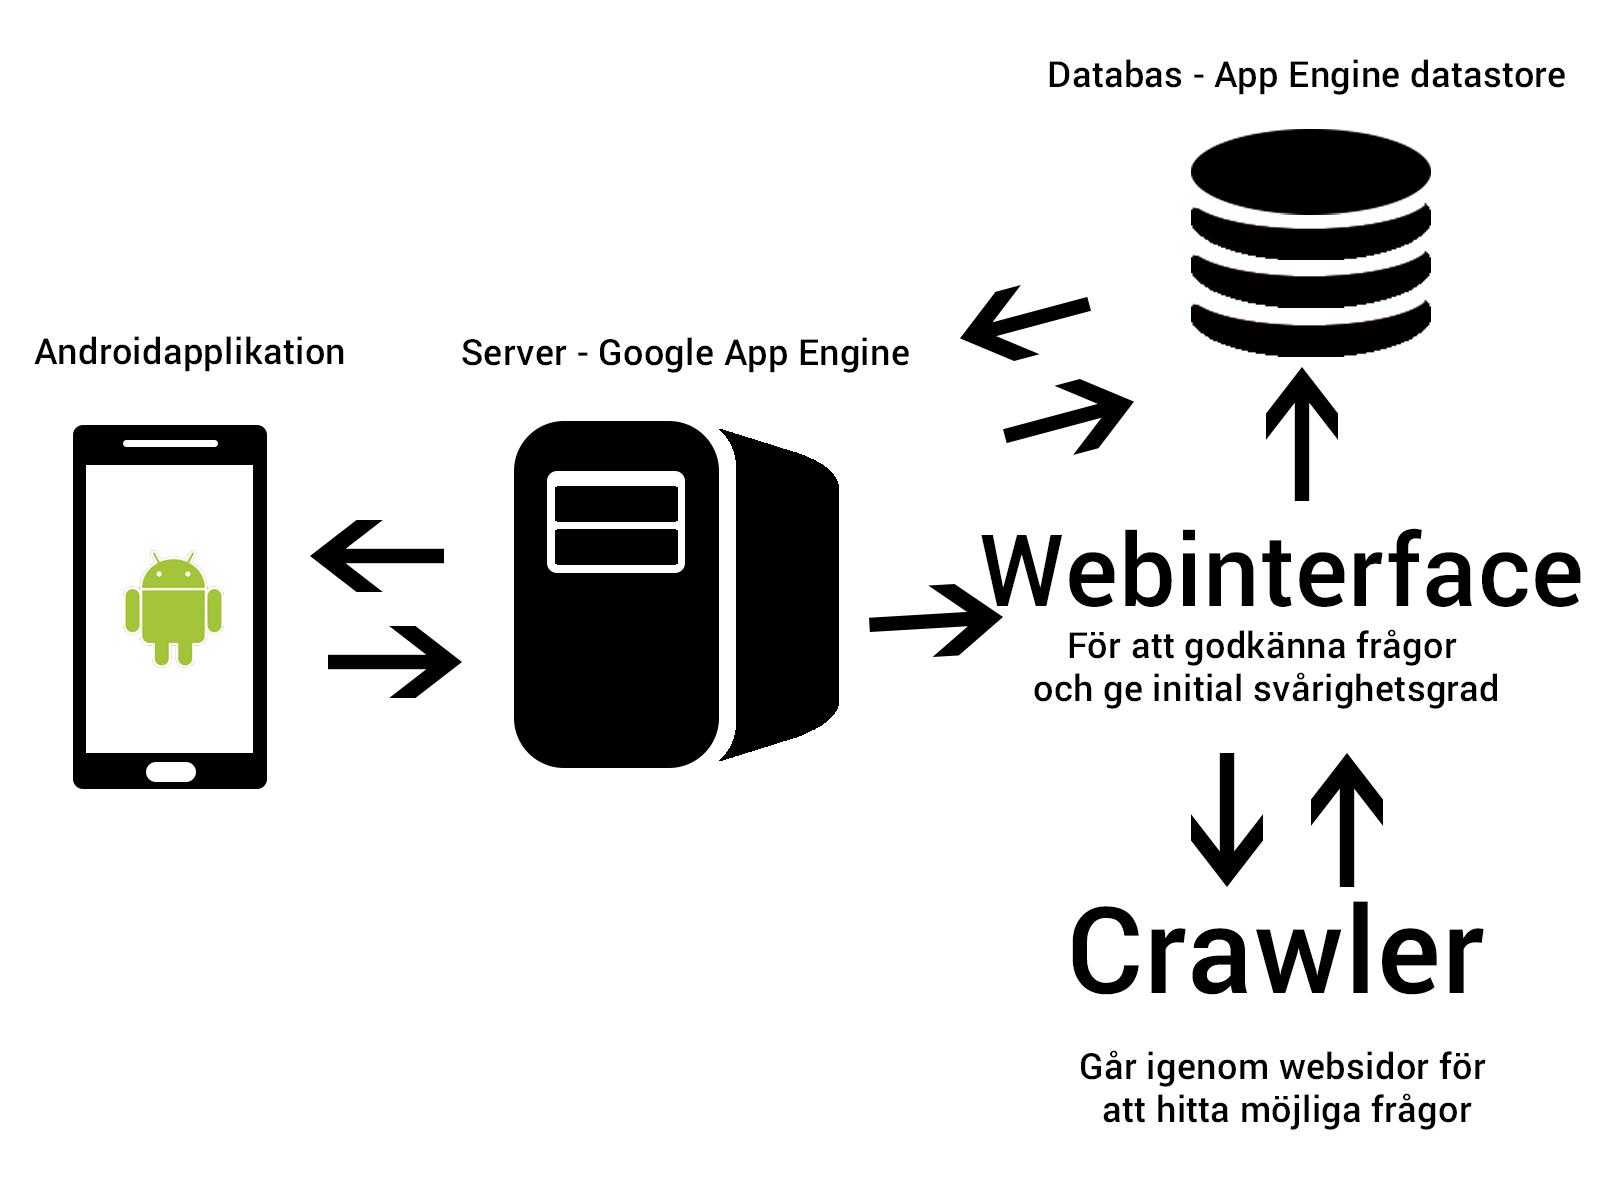
\includegraphics[width = \textwidth]{systemstruktur.jpg} 
	\end{centering}
	\caption{\textit{Illustration av systemstrukturen}}
\end{figure} 

\subsubsection{Androidapplikationen}
Androidapplikationen, klienten i systemet, är själva spelet som utvecklats. Det är den del av systemet som användaren interagerar med båda visuellt och funktionellt.

När det är den aktuella spelarens tur får hen en chunk med sex frågor och dess svar (årtal) från systemets server. Svaren är gömda för användaren under rundans gång och används endast av klienten för att rätta svaren från spelaren. När spelaren är färdig med sin runda och klienten har rättat svaren så skickas dessa tillbaka till servern där de lagras i matchens historik. 

\subsubsection{Server}
Klienten kommunicerar med en server som körs i Google App Engine. Servern är utvecklad i programspråket Go (Golang) \cite{golang}. Anledningen till att utvecklarna valde att skriva servern i Go är för att det, enligt utvecklarna, är ett simpelt språk med en syntax som liknar språk som utvecklarna använt tidigare. Servern agerar även som en brygga mellan klienten och den databas som används. När klienten kräver nya frågor till spelet kommunicerar servern med databasen. Databasen skickar frågor till servern som i sin tur skickar vidare till klienten. Utöver kommunikation till klienten och databasen används även servern för att köra crawlern som är den semi-automatiska informationshämtaren. Servern har också som uppgift att med jämna mellanrum köra fråge- och användarbalanseringssystemet som justerar svårighetsgraden på frågorna respektive spelarna i systemet. 

\subsubsection{Databas}
Databasen som servern kommunicerar med körs, likt servern, i App engine med biblioteket \textit{datastore}. Datastore \cite{datastore} är Google App Engines egna bibliotek för hantering och lagring av data vilket betyder att systemet, utan utvecklarnas assistans, hanterar all datalagring. Datastore har flera egenskaper som bidrar till en enklare utveckling av resterande delar för projektet. Med tanke på att Datastore är ett bibliotek från App Engine så medföljer dess skalbarhet som skalar beroende på behovet. Med Datastores inbyggda hjälpmedel för redundans kan data lätt replikeras till flera datacenter. \\
Datastore hanterar datalagring med både SQL och noSQL. Med Datastore behöver utvecklarna inte oroa sig över hur sökning och borttagning sker i databasen. Detta kan förklaras med faktumet att Datastore inte använder sig a schemas som en databas i exempelvis SQL. Sökning i databasen är också effektivt tack vare den solida sökmotorn som biblioteket tillhandahåller.

\subsubsection{Crawler} \label{crawler}
Inbyggt i servern finns en form av crawler som hanterar semi-automatisk informationshämtning av frågematerial. Hela systemet syftar till att via en given länk läsa igenom den länkade sidan och dess undersidor för att hitta information som passar som frågor för spelet. 

Sidor som har visat sig vara relativt enkla att läsa in är Wikipedias undersidor av typen listningssidor. Den här typen av sidor har en punktlista med årtal samt en beskrivande mening av det årtalet inom den kategori som Wikipediasidan handlar om. Ett exempel är sidan som listar datorspelsår: Som återfinns vid denna  \textbf{\href{http://sv.wikipedia.org/wiki/Lista_\%C3\%B6ver_datorspels\%C3\%A5r}{länk.}} 
Vid inläsning av den här typen av sida separeras helt enkelt varje $<$li$>$-element där ett bindestreck eller kolon förekommer och därefter sparas varje kombination av årtal och händelse i ett temporärt cache.

När alla  händelser har lästs in i cachet presenteras de inlästa händelserna en i taget i ett webinterface. Webinterfacet visar ett årtal, en fråga samt fyra knappar. Knapparna anger svårighetsgrad lätt, medel eller svår samt ett alternativ för att ta bort den aktuella frågan helt.

\begin{figure}[H]
	\begin{centering}
	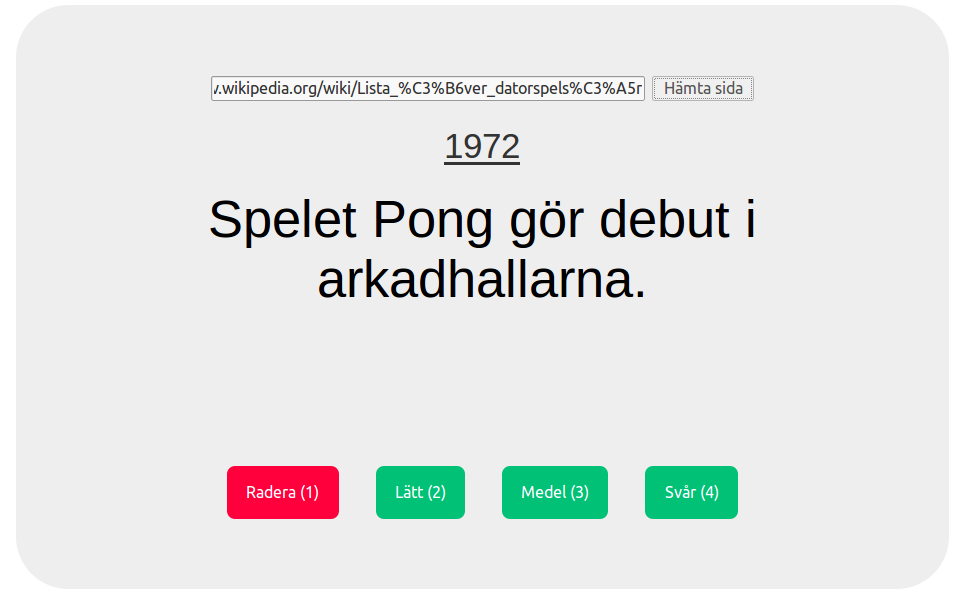
\includegraphics[width=\textwidth]{crawler} 
	\end{centering}
	\caption{\textit{Webinterface för crawlern}}
\end{figure}

De fyra knapparna är mappade till siffrorna 1-4 på tangentbordet för att det ska gå snabbt att klicka igenom frågorna. Texten är också redigerbar för att administratören snabbt ska kunna justera grammatiska fel.

\subsubsection{Användare}
Det finns två sorters användare som kan interagera med systemet.\\
\newline
\textbf{Administratörer} \label{admins}
Administratörerna är ansvariga för underhållet och utvecklingen av systemet. Administratörerna har den högsta typen av tillgång till systemet för att kunna utföra dessa uppgifter. I underhåll innefattas att felsöka och åtgärda funna fel men också uppföljning av rapporterade fel som skickas in av spelare. En vital uppgift som administratörerna har förutom den allmänna underhållet och utvecklingen av systemet är att godkänna informationen som hämtas av crawlern. Detta är för att se till att frågorna följer den struktur som administratörerna finner lämplig.\\
\newline
\textbf{Spelare}\\
Spelarna är den typen av användare som har en begränsad åtkomst till systemet. Spelarna kan endast komma åt systemet genom klienten och kan interagera med själva spelet. Detta betyder att en vanlig spelare inte kan finna information som ligger \textit{under huven} på systemet. Detta är delvis en säkerhetsåtgärd som är till för att den vanliga användaren inte, av misstag, eller med flit kunna komma åt systemets vitala delar och alternera dessa. Användaren kan kommunicera med administratörerna genom att skicka felrapporter om spelet skulle bete sig konstigt eller om några buggar har funnits.

\subsubsection{Balanseringssystemet} \label{balanseringssystemet}
Balanseringssystemet syftar till två saker, dels till att justera svårighetsgraden på frågorna som finns i databasen och dels till att justera spelarnas svårighetsnivå. 

Det finns alltså två separata nivåsystem i applikationen. Varje fråga i databasen har ett siffervärde för dess svårighetsgrad, ju högre siffra, desto svårare fråga. På liknande vis har också varje användare en svårighetsgrad som lagras som ett siffervärde i spelarens profil. Syftet med dessa poäng är i det stora perspektivet att få spelet att servera så rättvisa och roliga matcher som möjligt för spelarna. 

\paragraph{Balansering av frågorna}

Frågornas svårighetsnivå justeras beroende på hur spelarna i matchen svarar på frågan. En fråga som det ofta svaras fel på ökar i svårighetsnivå allt eftersom fler spelare svarar fel. Svårighetsnivån är helt bunden till frågan i sig och finns alltså kvar mellan matcherna.

En frågas svårighetsnivå har ingenting med någon form av poängräkning att göra. Svårighetsnivån på frågorna finns till för att vid en matchstart kunna jämföras mot spelarnas svårighetsnivå, på så vis avgör spelet om frågan ska skickas till spelarna eller inte. Det handlar alltså helt och hållet om att spelet ska presentera frågor som är lagom svåra för spelarna, så att spelet blir lagom utmanande och maximalt roligt.

Om en spelare med låg nivå svarar rätt på en fråga så justeras frågans svårighetsgrad ner, ju högre nivå frågan har, desto större nedjustering sker. En spelare med hög nivå påverkar inte frågorna lika mycket som en spelare med låg nivå. Det här beror på att om en spelare med låg nivå svarar rätt på en svår fråga så är nivån på frågan förmodligen mycket mer felaktig än om en avancerad spelare svarat rätt på samma fråga. 

\paragraph{Balansering av spelarna}

Spelarnas svårighetsnivåer justeras också efter avslutad match. Den här balanseringen går i stora drag till så att den vinnande spelaren tar poäng av den förlorande spelaren. Om den vinnande spelaren redan ligger på högre nivå än den förlorande så tar denne väldigt lite poäng från den förlorande. I det motsatta fallet tar istället den vinnande spelaren mycket poäng från den förlorande. Hur mycket poäng som faktiskt tas baseras på skillnaden i nivå mellan spelarna. 

Inspiration till den här sortens balansering kommer bland annat från Counter-strike: GO \cite{cs} som använder sig av Elo\cite{elo}. 

Balanseringen i \textbf{VÅRT SPEL} ansågs vara tillräckligt bra med Elo för att användningen av Glicko skulle uteslutas. Det är också förmodligen så att ett spel som schack eller Counter Strike behöver mer frekvent träning för att spelaren ska behålla sin nivå än ett frågesportspel som \textbf{VÅRT SPEL}. Allmänkunskap och historiekunskap är någonting som lättare förbättras i vardagen, än till exempel schacktaktik. 

I \textbf{VÅRT SPEL} sker balanseringen efter en avslutad match. När hela matchen är avslutad finns alla frågor från matchen samt respektive spelares svar i serverns cache. Efter att en vinnare har utsetts anropas balanseringssystemet och både frågenivåerna och spelarnivåerna justeras utifrån matchens utfall.

\begin{verbatim}
downDiff = int((1.0-(userRatio*questionRatio))*10.0)
\end{verbatim}

Kodsnutten ovan är ett exempel på en justering som sker om en spelare svarat rätt på den aktuella frågan. userRatio är ett värde mellan 0-1 på spelarens nivå (0 är nybörjare, 1 är avancerad). questionratio är ett värde mellan 0-1 på frågans nivå. downDiff är det värde som frågans nivå sänks med (mellan 0-10). 

\subsection{Avgränsningar}
Någon applikation för Windows och iOS fanns som en eventuell fortsatt utveckling efter Android men kommer inte att ske ty ett större fokus på en bra applikation till Android prioriteras. Spelet kommer troligtvis ha ett par kategorier för frågorna som ska finnas med i spelet, men dessa är ännu inte valda. 

I applikationen finns det många funktioner som skulle vara roliga och användbara, men inför projektet hade vi några funktioner som ansågs vara viktiga att ha med. Den viktigaste funktionen är att kunna hitta och spela en match. En funktion för att hitta och hantera vänner man har i spelet och även kunna se statistik över matcherna man spelat mot en vän. Dessa funktioner behöver så klart även implementeras på servern.

\subsection{Krav}
Systemet ska klara många spelare samtidigt, dock bara två per match. Någon speciell tak för antalet användare är inte bestämt ännu men med tanke på den otroligt solida grunden för skalbarhet som projektet står på kommer en siffra för antal spelare ganska snart kunna bestämmas. Eftersom App Engine används för servern så kommer det inte bli något problem med den enkla förklaringen att det är en tjänst som automatiskt skalar med hänsyn på belastning. \cite{appenginescalability}

Informationssökaren ska tillsammans med den administrativa kontrollen ge frågor som håller hög kvalitet. En hög kvalitet betyder frågor som är relevanta och som följer den strukturen vi har tänkt oss. Frågorna ska vara lätta att läsa, förstå och samtidigt befinna sig i det breda spektrumet av svårighetsgrader vi kommer ha i spelet. Sökaren för frågorna ska också vara så pass bra att den administrativa kontrollen går fort och att så lite som möjligt behöver korrigeras efter att frågorna har samlats in. För att applikationen inte ska kännas alldeles för repetitiv ska det finnas många frågor som dessutom är av varierande kategori. Det ska också finnas minst 1000 frågor sammanlagt.

Designen av applikationen är något som är väldigt viktigt för oss. Kravet i början var att ha en intuitiv, responsiv och snygg design. Eftersom applikationen gjordes för Android skulle den också följa dess designmönster Material Design \cite{MaterialDesign}.

\subsection{Utvärdering}
Planen är att en fungerande alfa eller betaversion av systemet ska färdigställas en rimlig tid innan projektet avslutas. I den här versionen ska användare ha möjlighet att ge feedback och att testa applikationen. Tack vare den feedback vi får från användarna så ska så många fel som möjligt justeras innan den skarpa versionen släpps.

Gränssnittet och användandet av applikationen kommer också att utvärderas med hjälp av think aloud \cite{thinkaloud} och en heuristic evaluering \cite{heruistic}.

\newpage
\printbibliography[title={Referenser}]
\end{document}